\chapter{LITERATURE REVIEW}

% Modify the following contents according to the literature review
\section{Previous Research and Designs}
\subsection{DetZero}
DetZero \parencite{ma2023detzero} is a LiDAR-based 3D object detection framework that introduces a \emph{long-term scene flow} approach. Instead of relying on only one or a few frames of LiDAR data, DetZero analyzes a long sequence of data. Although highly accurate, its reliance on long sequential LiDAR data results in very high latency and non-\emph{real-time} performance. DetZero employs \emph{batch processing} rather than \emph{stream processing}, which makes it completely unsuitable for \emph{real-time} decision-making within fractions of a second. Figure~\ref{fig:detzero_arch} shows the architecture of DetZero.

\begin{figure}[H]
  \centering
  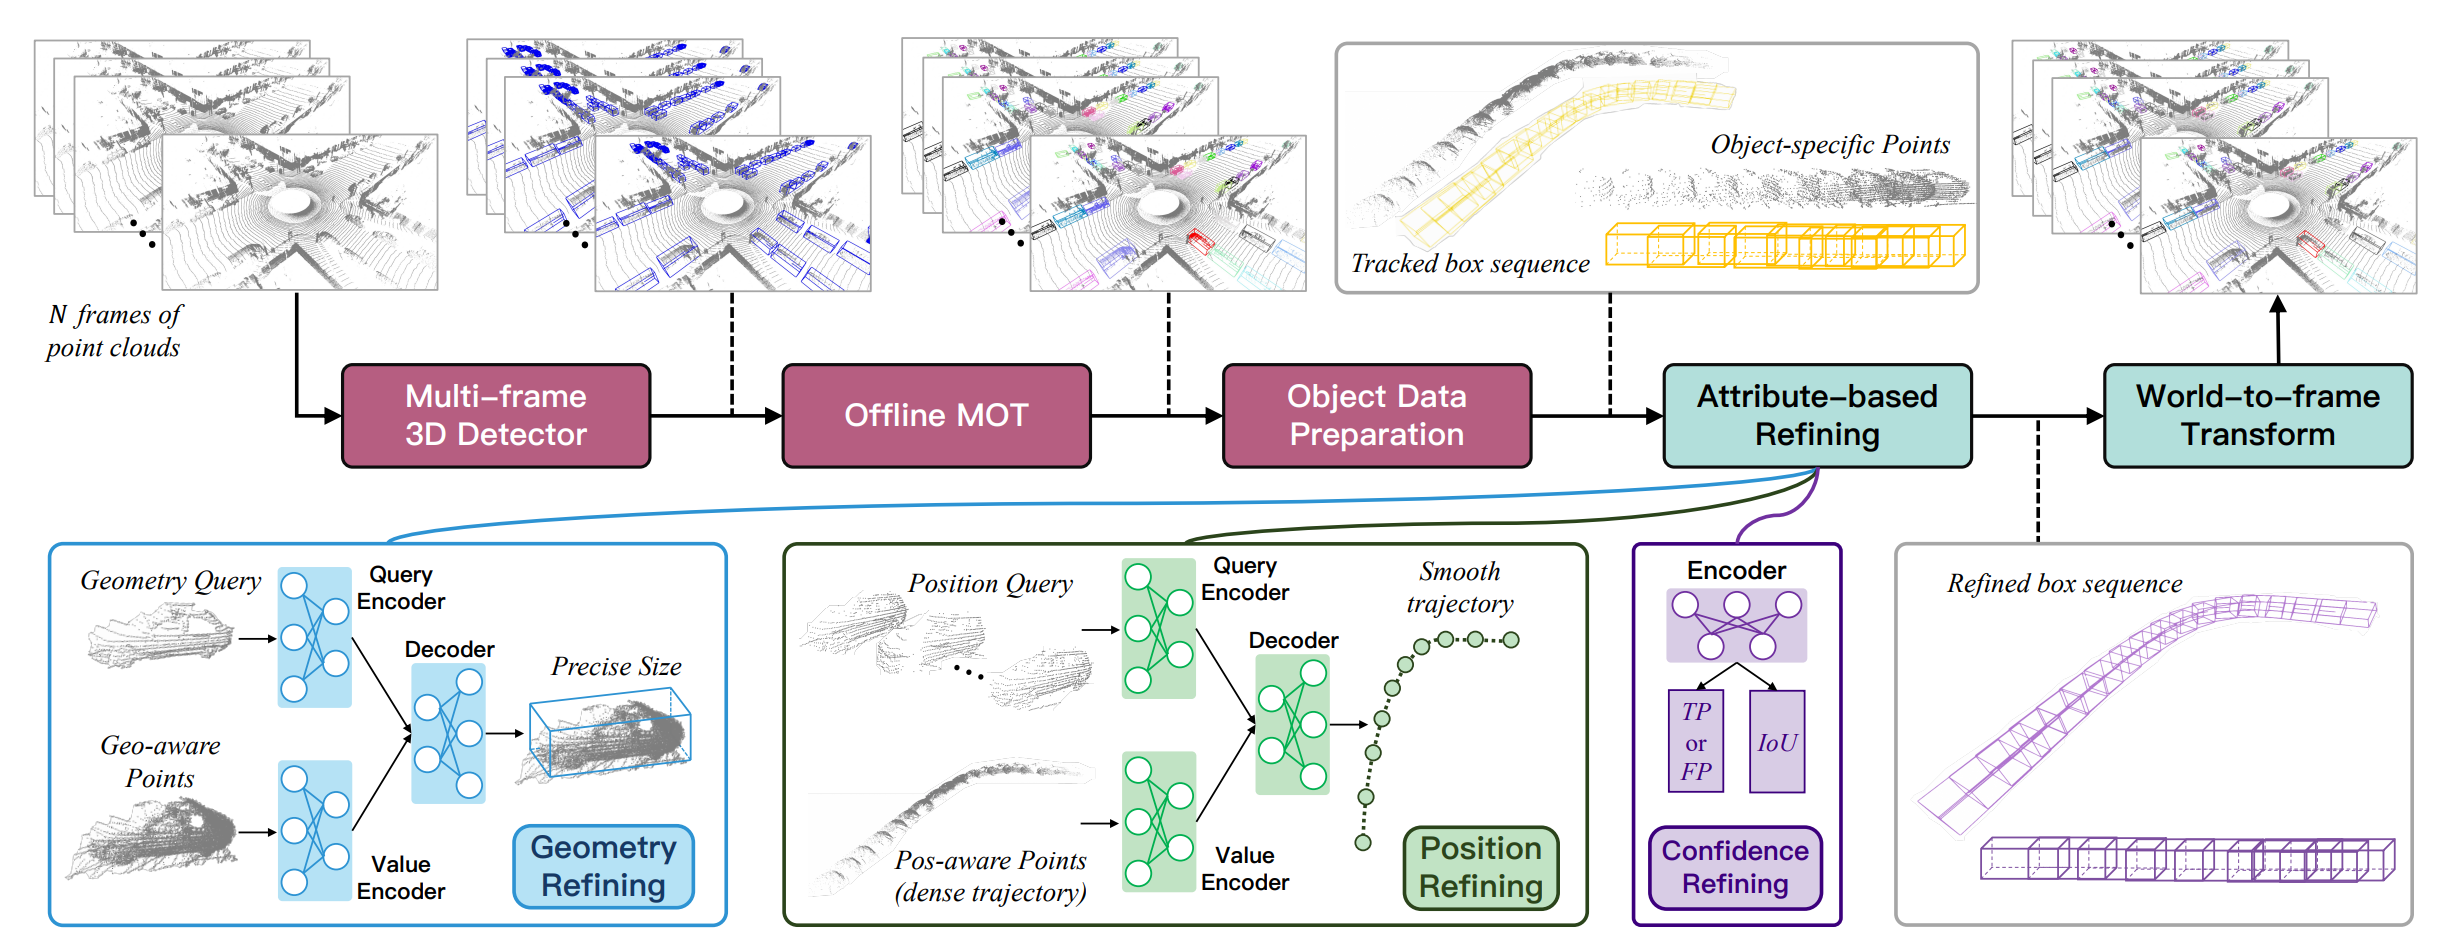
\includegraphics[scale=0.18]{gambar/detzero_architecture.png}
  \caption{DetZero System Architecture. DetZero introduces a multi-frame detector which aids in enhancing object point cloud geometry and detection quality.}
  \label{fig:detzero_arch}
\end{figure}

\subsection{PV-RCNN}
PV-RCNN converts the \emph{point cloud} into a series of 3D \emph{voxels} and applies 3D convolutional networks to extract features from the entire scene~\parencite{pvrcnn}. Figure~\ref{fig:pvrcnn_arch} shows the architecture of PV-RCNN. Essentially, PV-RCNN aims to perform in 3D what YOLO frameworks do in 2D. The major drawback of PV-RCNN lies in the voxelization step (transforming point clouds into 3D voxels/pixels), which consumes substantial computational resources. Additionally, PV-RCNN relies solely on the shape of an object to determine its class, which can lead to misclassifications between similarly shaped objects that differ significantly in color.

\begin{figure}[H]
  \centering
  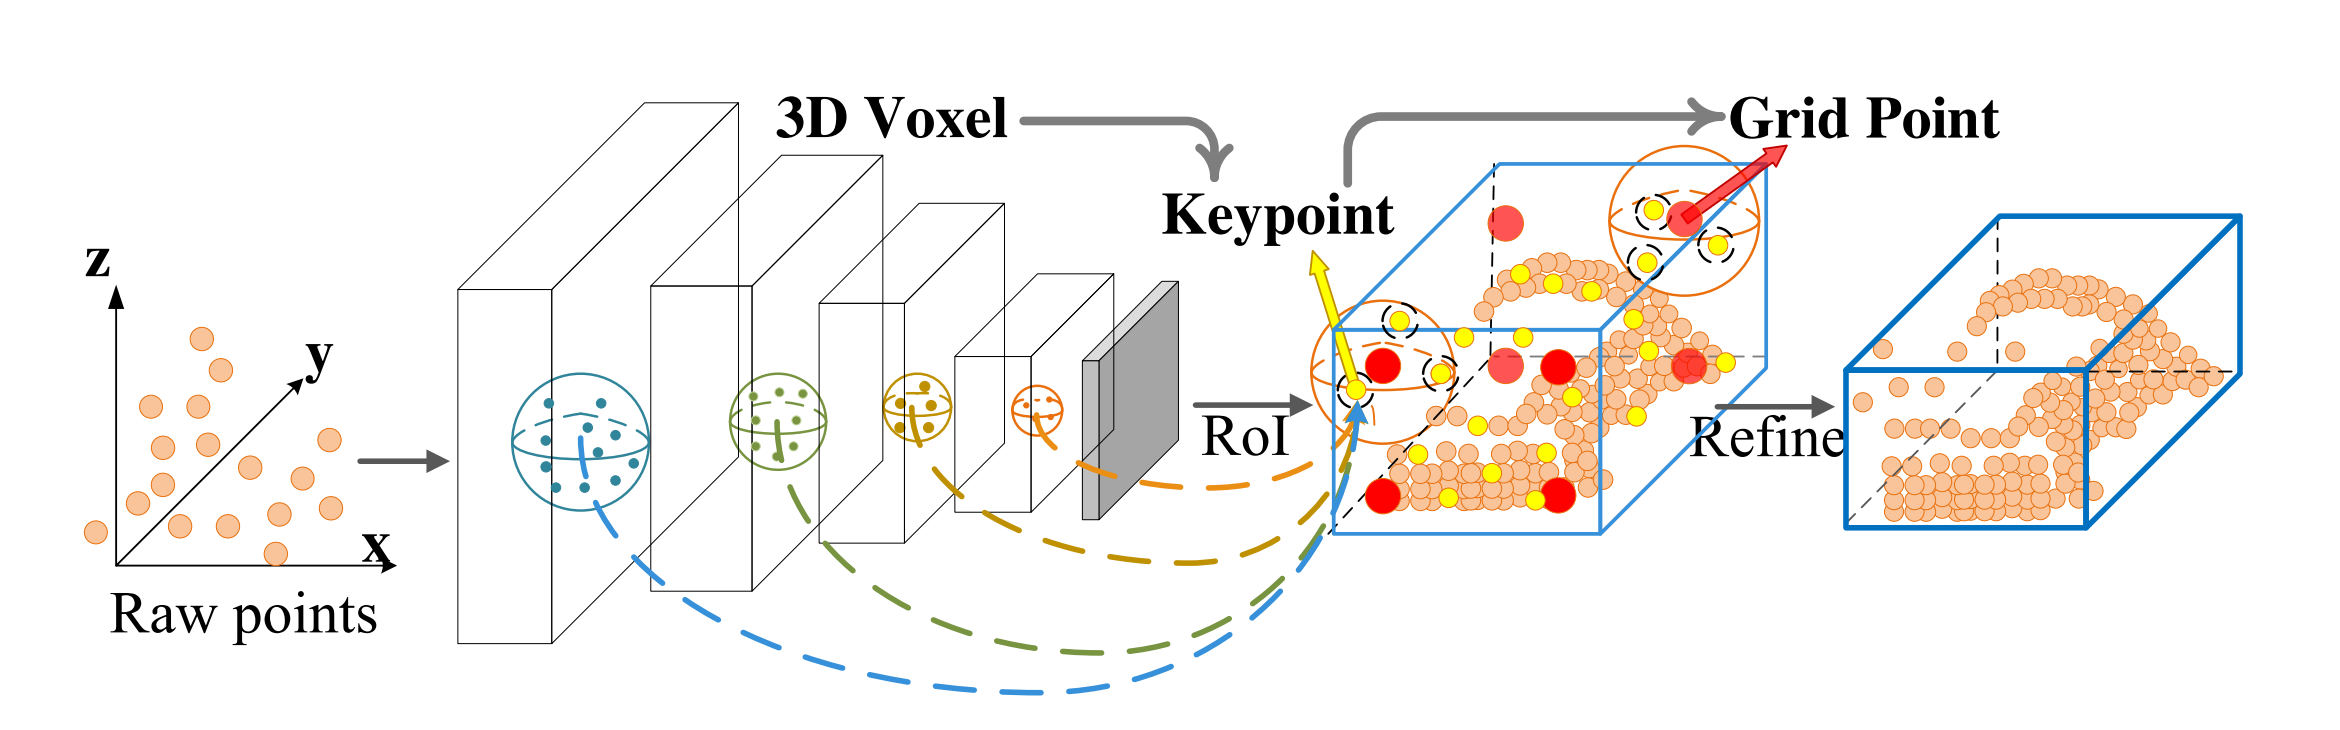
\includegraphics[scale=0.19]{gambar/pvrcnn_architecture.png}
  \caption{PV-RCNN System Architecture. PV-RCNN uses a voxel-to-keypoint 3D scene encoding to improve LiDAR-based 3D object detection.}
  \label{fig:pvrcnn_arch}
\end{figure}

\subsection{CenterPoint}
CenterPoint~\parencite{centerpoint} is an object detection framework that simplifies the detection head by predicting an \emph{objectsness heat-map} at the center of each instance, followed by a regression of size, yag, and velocity (a 3D modification of the anchor-box approach of YOLO versions up to YOLOv5). The absence of anchors reduces hyper-parameters and accelerates post-processing. CenterPoint employs a VoxelNet backbone with circular NMS and a 0.1m voxel grid, achieving 76.7 mAPH on Waymo LEVEL\_2, yet it needs 8 GB of GPU RAM plus 400 MB of CPU RAM and still takes 60 ms on an RTX-2080Ti in single-sweep mode, comfortably under the 40ms soft-real-time threshold on a 15W SoC. Because it ingests only one LiDAR sweep at a time, the lact of temporal smoothing causes bounding boxes to flicker across frames, and by ignoring both camera and IMU data it remains sensitive to viewport changed and ego-motion drift. Figure~\ref{fig:centerpoint_arch} shows the architecture of CenterPoint.

\begin{figure}[H]
  \centering
  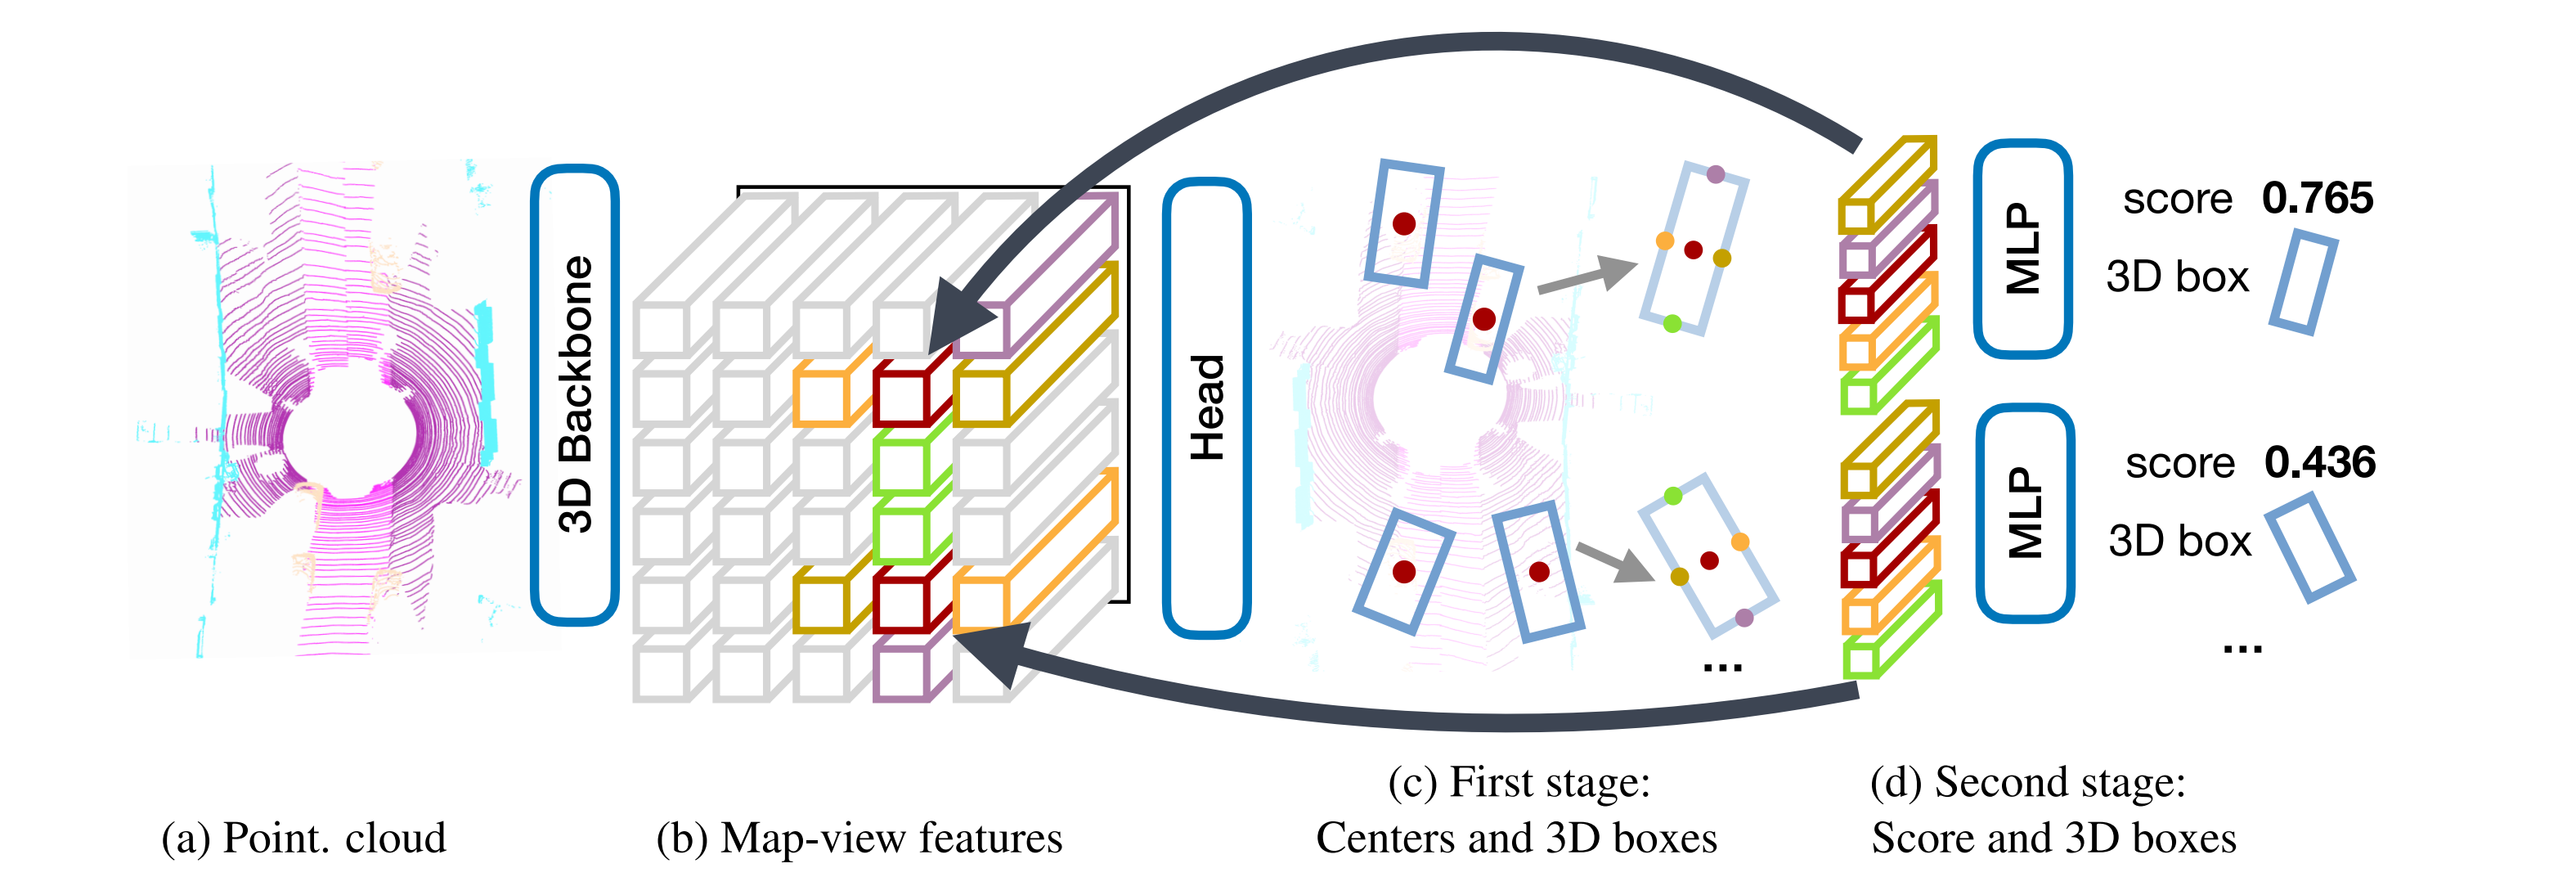
\includegraphics[scale=0.14]{gambar/centerpoint_architecture.png}
  \caption{CenterPoint System Architecture. CenterPoint uses a standard 3D backbone to extract features from LiDAR point clouds.}
  \label{fig:centerpoint_arch}
\end{figure}

\subsection{BEVFusion}
BEVFusion~\parencite{bevfusion} unifies camera and LiDAR features in a shared BEV raster by \emph{lifting} image features via predicted depth and then concatenating with LiDAR voxel features. Figure \ref{fig:dlio_arch} shows the architecture of BEVFusion. A shared transformer decoder refines the fused volume. BEVFusion ingests six 1920x1280 cameras plus one LiDAR sweep on the Waymo Open Dataset, relying on a dual-backbone that couples a Swin-T vision transformer with a VoxelNet LiDAR encoder and fuses their features thorugh deformable attention, achieving 78.9 mAPH on Waymo LEVEL\_2, but only after 120 ms on a pair of A100 GPUs that together drew about 200W. BEVFusion requires a power budget roughly two orders of magnitude beyond what an embedded SoC can spare, and the heavy transformer layers together with the dense bird's-eye-view (BEV) grid make on-device streaming impractical. Moveover, the system insists on six precisely calibrated cameras, locking users into a rigid sensor suite that complicates integration on smaller, more flexible autonomous platforms.

\begin{figure}[H]
  \centering
  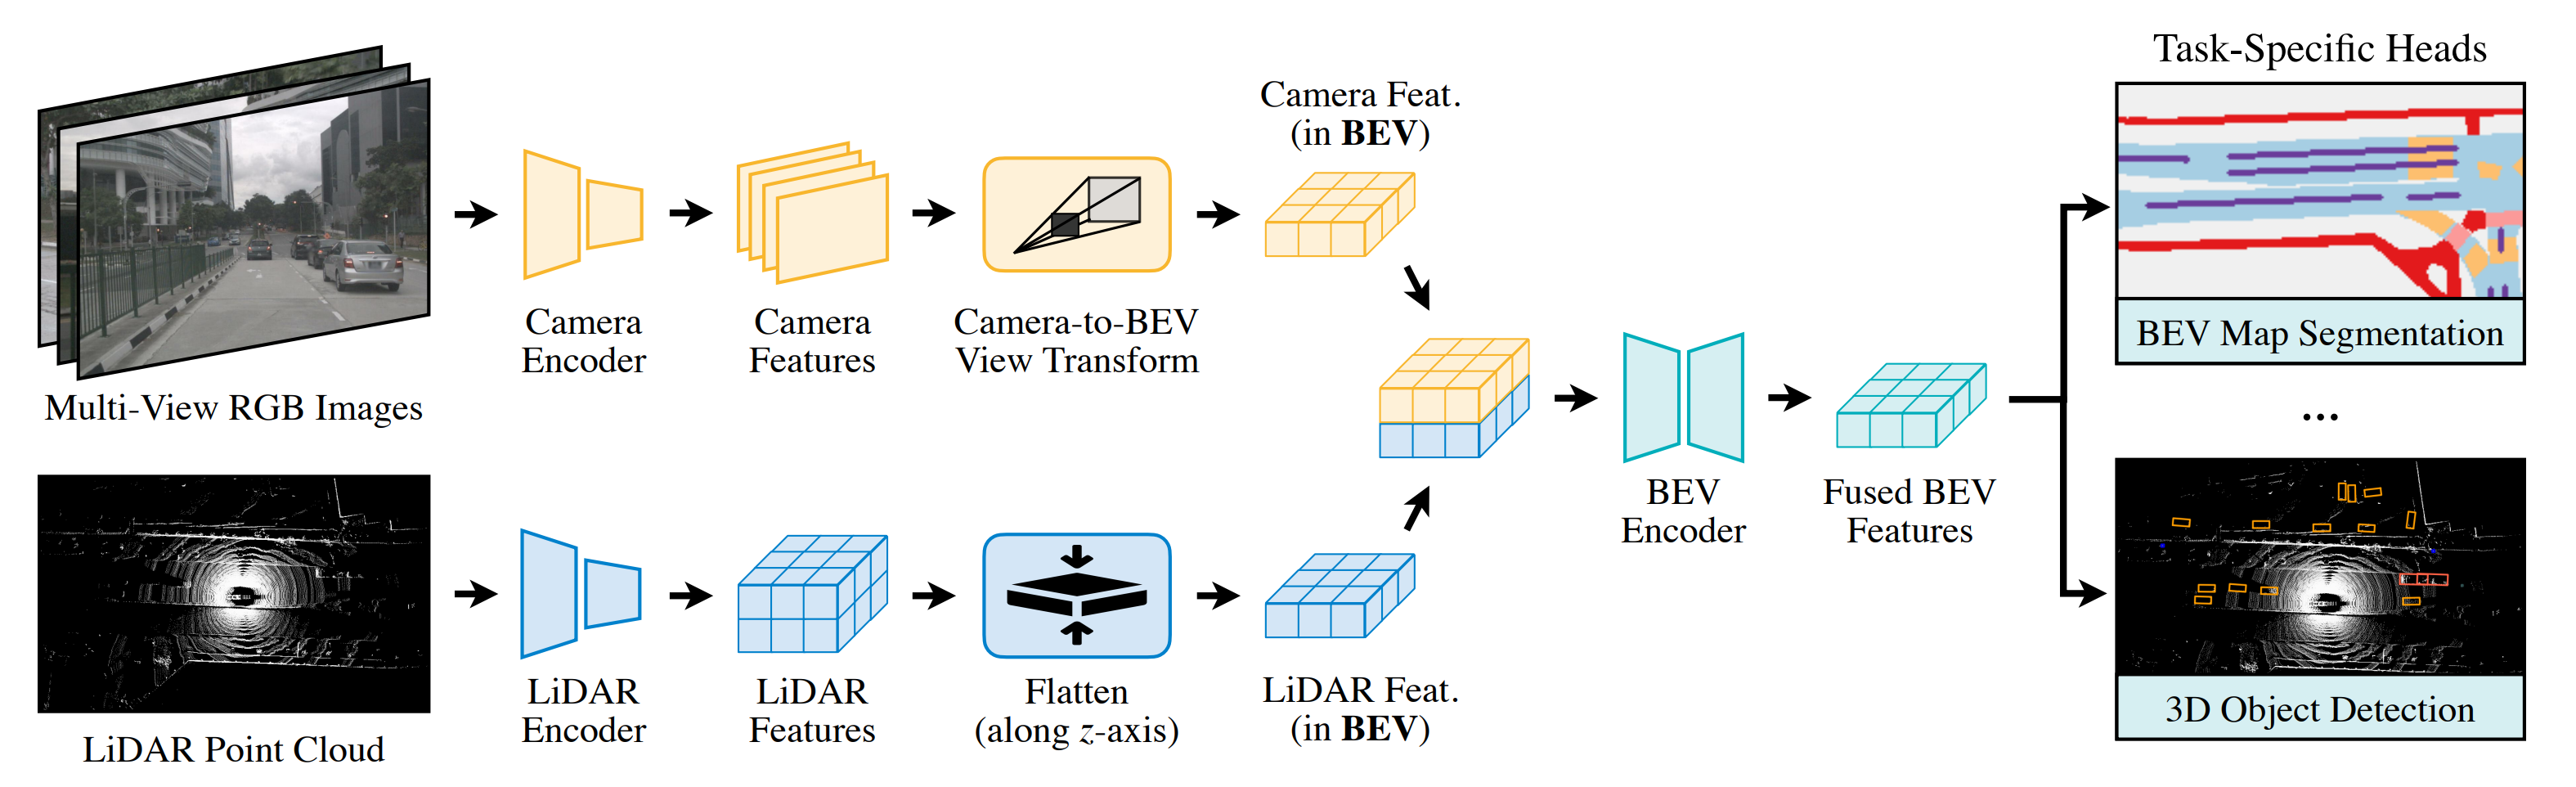
\includegraphics[scale=0.14]{gambar/bev_architecture.png}
  \caption{BEVFusion System Architecture. BEVFusion extracts camera and LiDAR features in a shared BEV raster by \emph{lifting} image features via predicted depth and then concatenating with LiDAR voxel features.}
  \label{fig:dlio_arch}
\end{figure}


\subsection{DLIO}
\emph{Direct LiDAR-Inertial Odometry} (DLIO) is an approach for ego-motion estimation, which is the process of determining the movement and orientation of a sensor (and the vehicle it is mounted on) over time. DLIO specifically combines data from a LiDAR sensor with data from an \emph{Inertial Measurement Unit} (IMU) to achieve accurate and robust trajectory estimation \parencite{dlio}. The word "Direct" in DLIO refers to the method used to process \emph{point cloud} data. Unlike "indirect" or feature-based methods, which first extract geometric features such as planes, edges, or corners from the \emph{point cloud} and then match these features across scans, the \emph{direct} method works directly on the raw point data. This method attempts to find the optimal transformation (rotation and translation) to align \emph{point clouds} from one time step to the next by directly minimizing geometric error. This approach avoids the feature extraction step, which can be computationally expensive and may discard useful information. Figure \ref{fig:dlio_viz} shows the architecture of DLIO.

\begin{figure}[H]
  \centering
  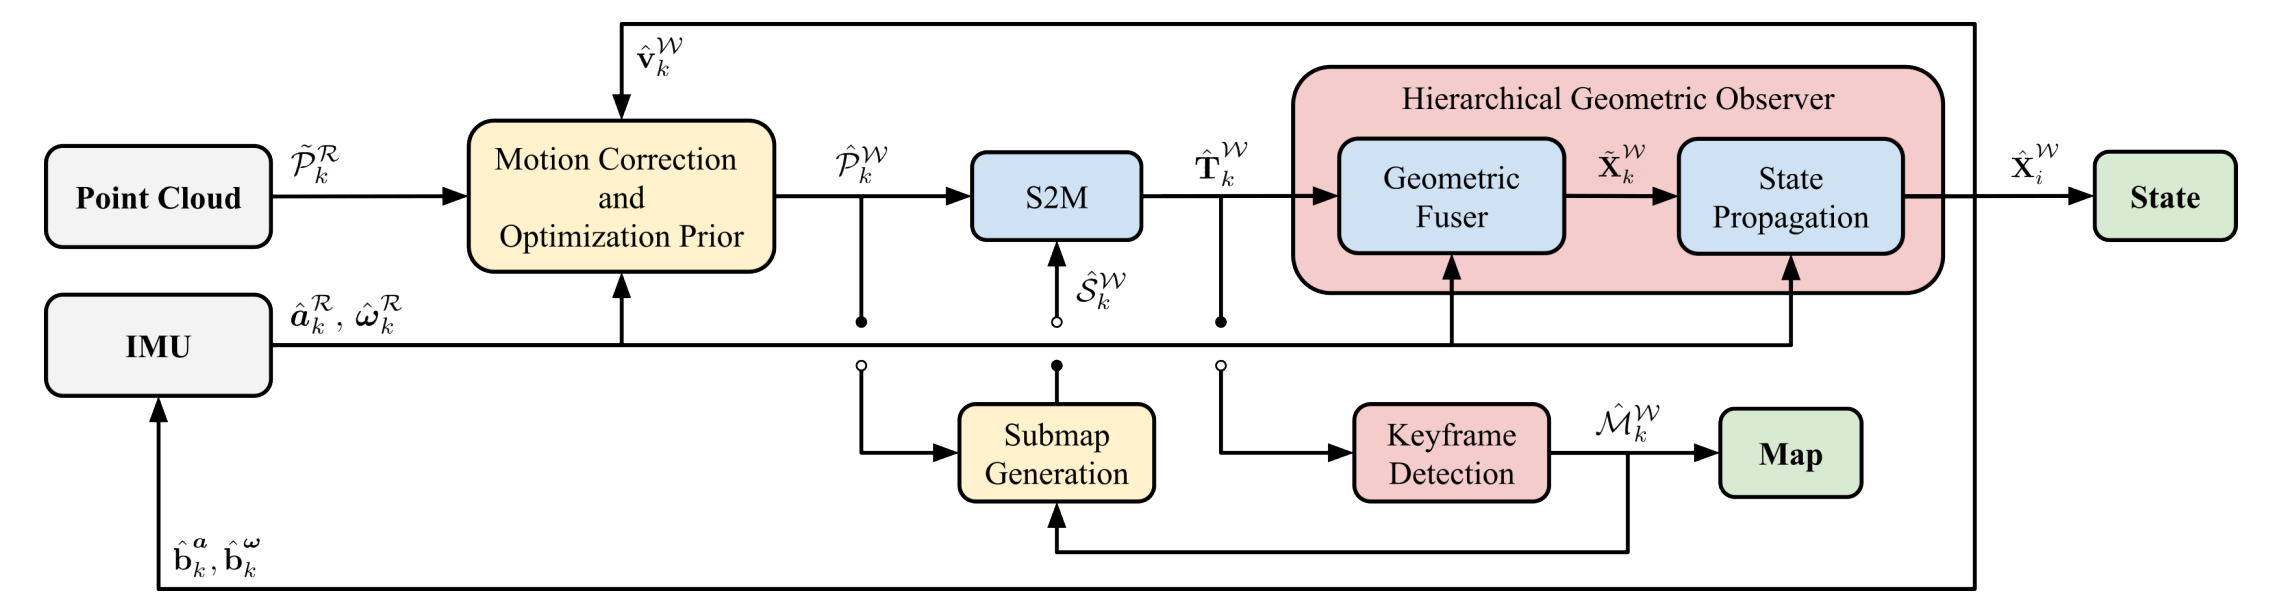
\includegraphics[scale=0.2]{gambar/dlio_architecture.png}
  \caption{DLIO System Architecture. DLIO provides a lightweight architecture that combines motion correction and prior construction into a single step, whilst also removing the computationally expensive scan-to-scan module previously required for LiDAR-based odometry.}
  \label{fig:dlio_viz}
\end{figure}

\subsection{Gap Analysis vs RT-LIVO2DM}

The following tables visualizes both the performance and qualitative gaps between each existing methods. Table~\ref{tab:gap_perf} lists mAPH on the Waymo Open Dataset validation split alongside latency and power, which highlights the divide between high-accuracy systems with hundreds of watts power requirement versus lightweight systems that sacrifice perception fidelity. Table~\ref{tab:gap_attrs} explains the major differences in sensor fusion and output attributes of each approach, with some methods relying on only LiDAR while others combine camera and LiDAR data, and some methods offer 3D maps while others do not.
% Table 1: Performance and Resource Footprint
\begin{table}[h!]
    \centering
    \caption{Gap Analysis: mAPH, Latency/FPS and Power}
    \begin{tabular}{lccc}
        \toprule
        \textbf{Method} & \textbf{mAPH} & \textbf{Latency / FPS} & \textbf{Power} \\
        \midrule
        DetZero     & 82.7 & 800 ms / 1.3 FPS & 300 W \\
        PV-RCNN     & 64.8 & 150 ms / 6.7 FPS & 250 W \\
        CenterPoint & 76.7 & 60 ms / 16 FPS  & 225 W \\
        BEVFusion   & 78.9 & 120 ms / 8 FPS  & 200 W \\
        DLIO        & —    & 8 ms / 125 FPS  & 45 W  \\
        \midrule
        \textbf{RT-LIVO2DM (Target)} & \textbf{$\geq 50$} & \textbf{$\leq 40$ ms / $\geq 25$ FPS} & \textbf{15--30 W} \\
        \bottomrule
    \end{tabular}
    \label{tab:gap_perf}
\end{table}

% Table 2: Sensor-Fusion & Output Capabilities
\begin{table}[h!]
    \centering
    \caption{Gap Analysis: Sensor Fusion and Output Attributes}
    \begin{tabular}{lccc}
        \toprule
        \textbf{Method} & \textbf{Color + IMU} & \textbf{Objects} & \textbf{3D Map} \\
        \midrule
        DetZero     & No  & Yes & Yes \\
        PV-RCNN     & No  & Yes & No  \\
        CenterPoint & No  & Yes & No  \\
        BEVFusion   & Yes & Yes & Yes \\
        DLIO        & Yes & No  & Yes \\
        \midrule
        \textbf{RT-LIVO2DM (Target)} & Yes & Yes & Yes, with Color \\
        \bottomrule
    \end{tabular}
    \label{tab:gap_attrs}
\end{table}

\section{Theoretical Foundations}

\subsection{LiDAR (\emph{Light Detection and Ranging})}

\begin{figure}[H]
  \centering
  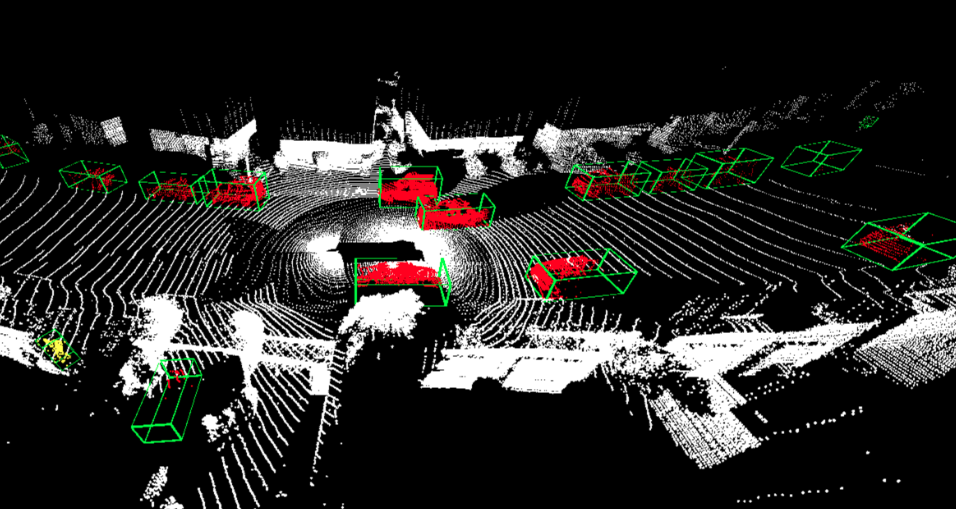
\includegraphics[scale=0.35]{gambar/waymo_lidar.png}
  \caption{Example of how LiDAR data is visualized, Waymo Open Dataset}
  \label{fig:waymo_lidar}
\end{figure}

LiDAR, short for \emph{Light Detection and Ranging}, is an active remote sensing method using pulsed laser light to measure distances from a fixed reference point~\parencite{lidar_principles}. It uses the \emph{time-of-flight} (ToF) principle (the same principle used in RADAR and SONAR systems), where a laser pulse (usually in infrared wavelength) is emitted toward an object and the time taken to return is used to determine the precise distance between the sensor and the object in which the light bounced on using the following equation:

\begin{equation}
  \label{eq:lidar_tof}
  d = \frac{c \cdot t}{2}
\end{equation}

Where:

\begin{itemize}
  \item $d$ is the distance to the object
  \item $c$ is the speed of light $ \approx 299.792 Km/s $
  \item $t$ is the round-trip time of the laser pulse
\end{itemize}

The data produced by LiDAR sensors is a collection of point data called a \emph{point cloud}, as shown in Figure~\ref{fig:waymo_lidar}. Each point in the \emph{point cloud} represents a single laser reflection and has 3D spatial coordinates (x, y, z). On some LiDAR devices, each point also carries additional information such as reflection intensity, which can help distinguish materials with different reflectivity. The main advantage of LiDAR compared to cameras is its ability to directly and accurately (without guesswork) measure depth, which can provide reliable information about 3D shapes and structures. Since LiDAR is a sensor that emits its own light source, its performance is not affected by external lighting conditions; LiDAR can function well at night as well as under bright sunlight.

Although it has advantages in 3D perception, LiDAR also has limitations in capturing rich color and texture information as a camera does. This makes it difficult to differentiate objects with similar shapes but different visual appearances (for example, a pedestrian and a traffic sign pole from certain angles). In addition, LiDAR performance can degrade significantly in weather conditions that produce many airborne particles such as very thick fog, rain, or snow.

\subsection{Computer Vision}
Like many AI implementations, developing a \emph{Computer Vision}-based system involves designing a \emph{model}—an algorithm that holds the foundational knowledge required to translate raw input into meaningful conclusions. A \emph{classifier} is the most suitable model type for object detection tasks, as it determines the object \emph{class} from given input data. The main goal of \emph{Computer Vision} implementation is to extract high-level information from images without human intervention. Applications include face recognition, motion detection in video, medical imaging, and more. Contemporary \emph{Computer Vision} approaches are dominated by \emph{Deep Learning} techniques~\parencite{deeplearning_lecun}, which continue to evolve rapidly at the time of writing.

% \emph{Deep Learning} (DL) adalah sebuah cabang dari \emph{Artificial Intelligence}/AI yang menggunakan jaringan saraf tiruan berlapis banyak (\emph{deep neural network}) untuk mempelajari representasi data. Efektivitas DL telah terdemonstrasi dalam beragam aplikasi, meliputi pengenalan citra, pemrosesan bahasa alami, dan deteksi objek.

\begin{figure}[H]
  \centering
  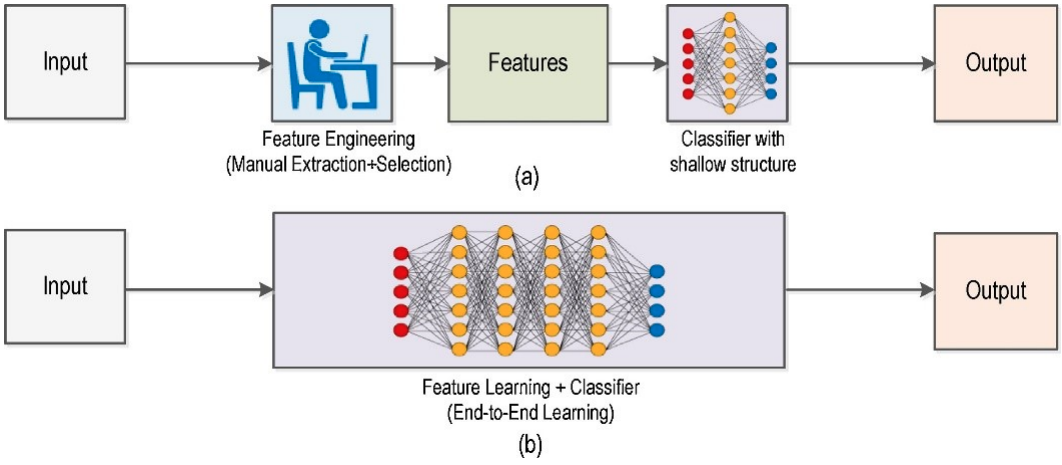
\includegraphics[scale=0.35]{gambar/traditional_vs_deep_learning_cv.png}
  \caption{(a) Traditional \emph{Computer Vision} approach vs. (b) \emph{Deep Learning}-based approach.}
  \label{fig:traditional_vs_deep_learning_cv}
\end{figure}

Visualized through Figure~\ref{fig:traditional_vs_deep_learning_cv}, before the advent of \emph{Deep Learning}, raw image data had to be manually interpreted into features (e.g., color, texture, shape) using \emph{Feature Selection} (FS) algorithms. Models then analyzed these features rather than raw pixels.

However, FS algorithm development was time-consuming, especially with many classes to detect. Moreover, adding a new class often required manual algorithm redesign. \emph{Deep Learning} automates FS by learning feature representations during training, enabling complex object detection and differentiation across hundreds of classes. AlexNet is commonly regarded as the first implementation that automates Feature Extraction with a Deep Convolutional Neural Network (DCNN)~\parencite{alexnet}.

\subsection{YOLO Framework}

YOLO (\emph{You Only Look Once}) is a \emph{Deep Learning}-based object detection algorithm designed for real-time performance. Instead of pinpointing exact object locations, it predicts \emph{confidence} values indicating the likelihood of objects in image regions \parencite{yolo_review}. Originally built for speed, newer YOLO versions have improved in accuracy and precision. Figure~\ref{fig:yolo_history} shows the development history of YOLO algorithms.

\begin{figure}[H]
  \centering
  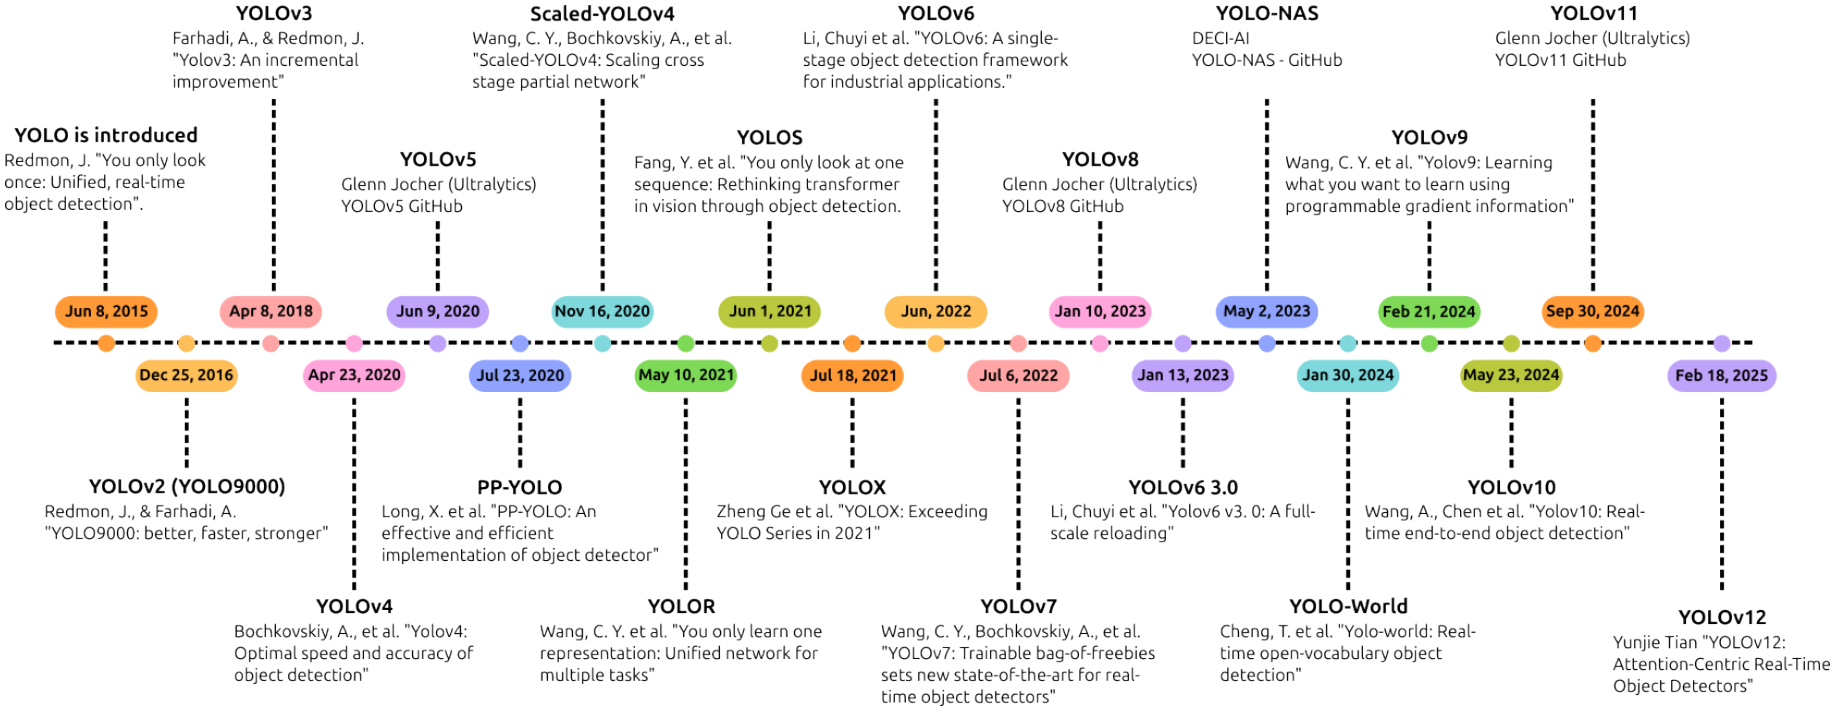
\includegraphics[width=\textwidth]{gambar/yolo_history.png}
  \caption{YOLO algorithm development history}
  \label{fig:yolo_history}
\end{figure}

Higher version numbers don't always indicate better performance. Some YOLO variants prioritize speed, others emphasize large-object detection, and some serve as experimental frameworks for new algorithmic techniques. Analysis shows YOLOv11 offers the best balance between accuracy and efficiency \parencite{yolo12_11_vs_others}. Ultralytics YOLOv11 is the latest version developed by Ultralytics. It improves both detection accuracy and inference speed over its predecessors. New features include multi-scale object detection, better small-object detection, and improved memory efficiency. Currently it is both more accurate and faster than the novel YOLOv12.

% \begin{figure}[H]
%   \centering
%   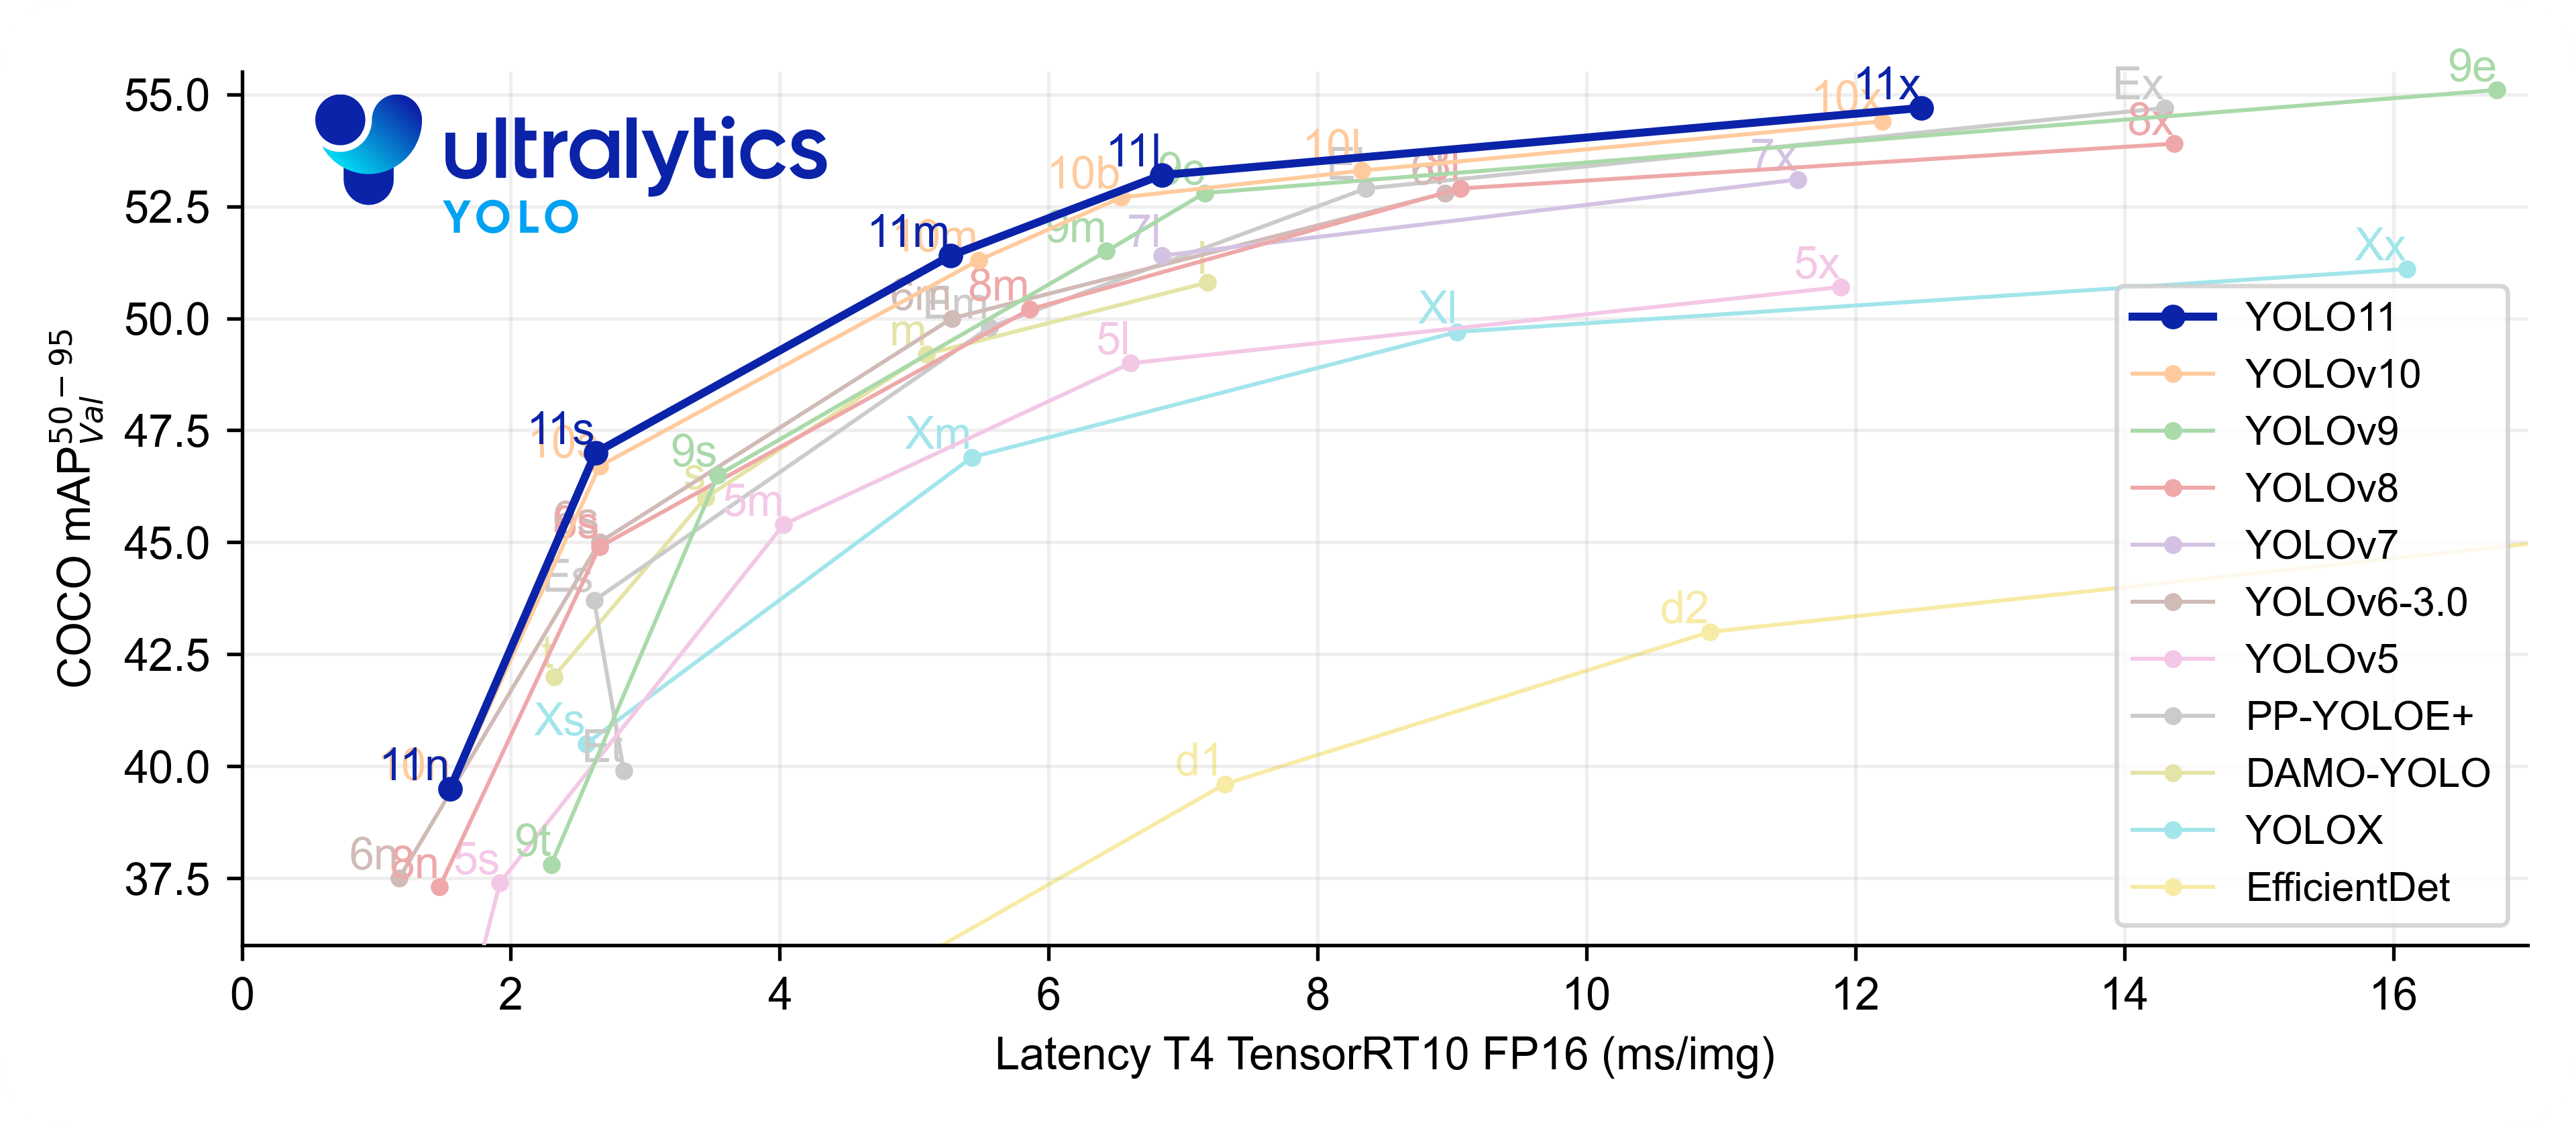
\includegraphics[width=\textwidth]{gambar/yolov11_performance.png}
%   \caption{YOLOv11 vs. other object detection algorithms \parencite{ultralytics2025yolo11}.}
%   \label{fig:yolov11_performance}
% \end{figure}

\subsection{Waymo Open Perception Dataset}

The Waymo Open Perception Dataset (WOPD) ~\parencite{Sun_2020_CVPR} is a publicly-available dataset provided by Waymo, an autonomous taxi company in the United States, a subsidiary of the Alphabet Group ~\parencite{waymo2025}. WOPD is a subset of the larger Waymo Open Dataset (WOD). WOPD is described as  having high resolution sensor data and labels for various tasks. The Waymo Open Perception Dataset is released through the official GitHub Repository~\parencite{waymo2025dataset}.

WOPD contains the following sensor data:

\sloppy
\begin{itemize}
    \item 1 mid-range LiDAR (\verb|T|)
    \item 4 short-range LiDARs (\verb|FRONT/F|, \verb|SIDE_LEFT/SL|, \verb|SIDE_RIGHT/SR|, \verb|REAR/R|)
    \item 5 cameras (\verb|FRONT/F|, \verb|FRONT_LEFT/FL|, \verb|FRONT_RIGHT/FR|, \verb|SIDE_LEFT/SL|, \verb|SIDE_RIGHT/SR|)
    \item Vehicle poses (\verb|IMU|)
\end{itemize}


Table~\ref{tab:wopd_full_specs_t} summarises the complete technical specification of every sensor and the pose attributes in the Waymo Open Perception Dataset.
Columns correspond to the five LiDAR units (TOP, F, SL, SR, R) and the five RGB cameras (F, FL, FR, SL, SR); the bottom block lists the synchronized 6-DoF vehicle pose, velocity, and global-timestamp auxiliary data that accompany every frame.

\begin{table}[h!]
  \centering
  \renewcommand{\arraystretch}{1.1}
  \small
  \caption{Transposed Sensor \& Pose Specifications. Values are taken from the official documentation for the Waymo Open Perception Dataset.}
  \label{tab:wopd_full_specs_t}
  \begin{tabular}{@{}lccccc@{}}
  \toprule
  \textbf{Attribute} & \textbf{T} & \textbf{F} & \textbf{SL} & \textbf{SR} & \textbf{R} \\ 
  \midrule
  \textbf{LiDAR} \\
  Beams & 64 & 16 & 16 & 16 & 16 \\
  Vertical Res. ($^\circ$) & 0.4 & 1.33 & 1.33 & 1.33 & 1.33 \\
  FOV (H × V) & 360 × 26.8 & 90 × 26.8 & 90 × 26.8 & 90 × 26.8 & 90 × 26.8 \\
  Range (m) & 0–75 & 0–20 & 0–20 & 0–20 & 0–20 \\
  Accuracy (cm) & $\pm$2 & $\pm$2 & $\pm$2 & $\pm$2 & $\pm$2 \\
  \midrule
  \textbf{Cameras (RGB)} & & & & & \\
  Resolution (px) & — & 1920×1280 & 1920×1280 & 1920×1040 & 1920×1040 \\
  HFOV ($^\circ$) & — & $\pm25.2$ & $\pm25.2$ & $\pm25.2$ & $\pm25.2$ \\
  VFOV ($^\circ$) & — & $\pm16.0$ & $\pm16.0$ & $\pm13.3$ & $\pm13.3$ \\
  \midrule
  \textbf{Pose / Auxiliary} \\
  Vehicle Pose & \multicolumn{5}{c}{6-DoF SE(3), position $\pm5$ cm, heading $\pm0.1^\circ$} \\
  Velocity & \multicolumn{5}{c}{3-DoF linear+angular, 10 Hz fused IMU/encoders} \\
  Timestamp & \multicolumn{5}{c}{64-bit µs, global clock $\le100$ µs error} \\
  \bottomrule
  \end{tabular}
\end{table}

Figure~\ref{fig:wopd_sensors} depicts the physical placement of these sensors on the roof-mounted mast, while Figure~\ref{fig:sensor_sync} quantifies the sub-millisecond hardware-level time alignment between LiDAR sweeps and camera exposures provided by WOPD.

\begin{figure}[H]
  \centering
  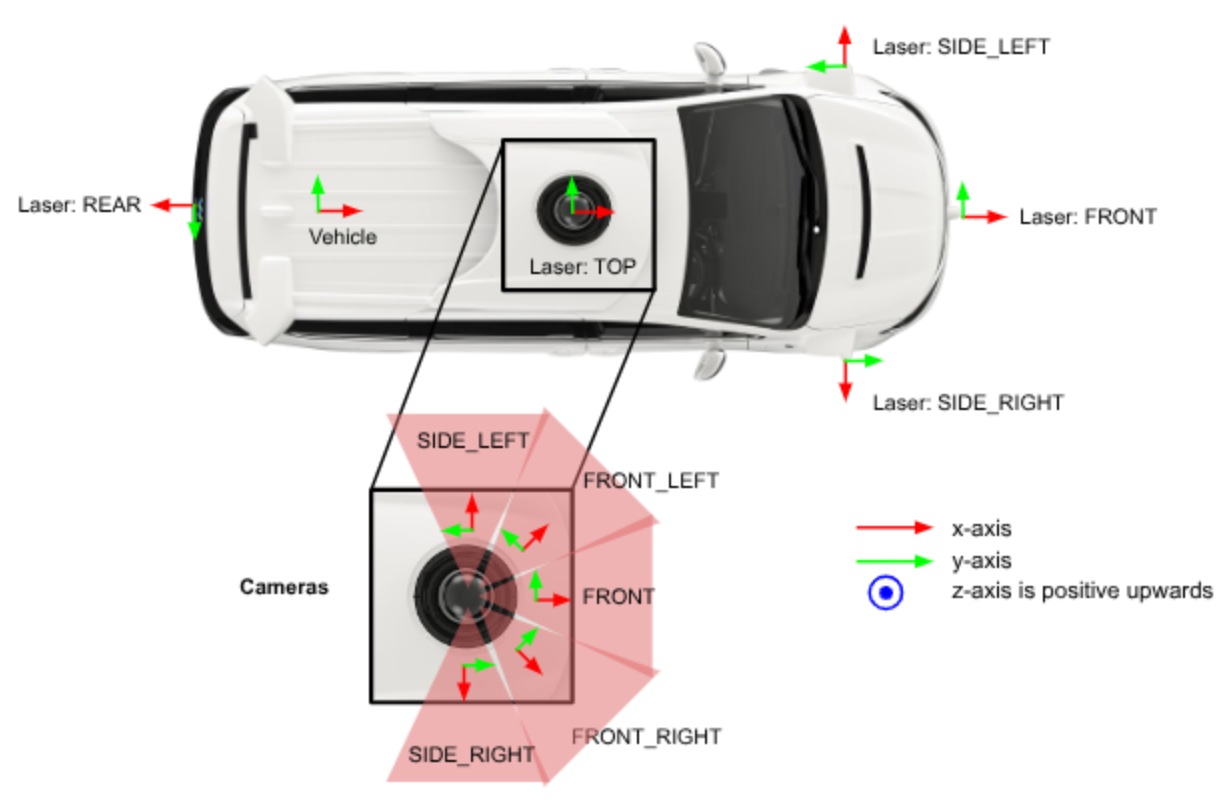
\includegraphics[scale=0.25]{gambar/wopd_sensors.png}
  \caption{Sensor layout and coordinate systems, WOPD}
  \label{fig:wopd_sensors}
\end{figure}

\begin{figure}[H]
  \centering
  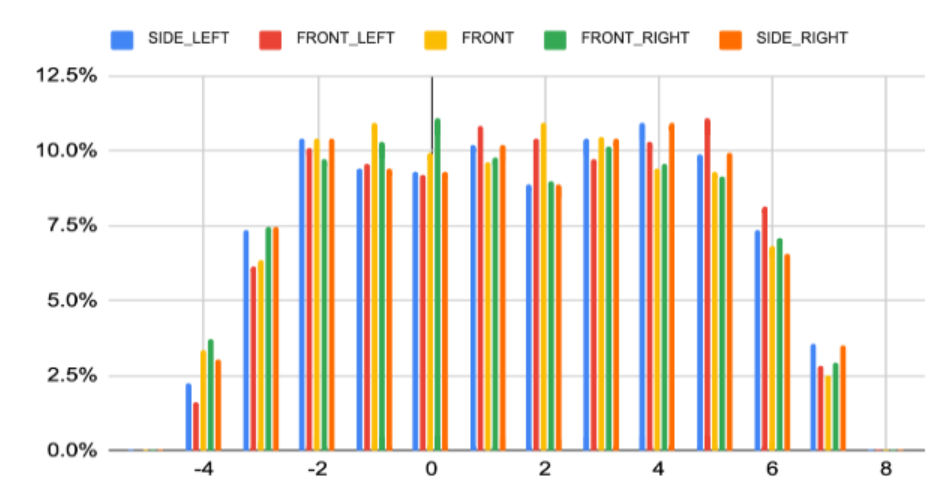
\includegraphics[scale=0.4]{gambar/sensor_sync.png}
  \caption{Camera-LiDAR synchronization accuracy}
  \label{fig:sensor_sync}
\end{figure}

\subsection{NVIDIA DRIVE and \emph{Edge Computing} in Autonomous Vehicles}

The implementation of \emph{Edge Computing} in autonomous vehicles relies entirely on high-performance computing hardware installed within the vehicle. This hardware, often referred to as the "brain" of the vehicle, must be capable of processing data from dozens of sensors and running complex AI algorithms within milliseconds. This hardware is fundamentally different from cloud server computers, as it must operate within strict constraints of power, heat, and size inside the vehicle, while also meeting very high automotive safety standards (ASIL – \emph{Automotive Safety Integrity Level}).

The NVIDIA DRIVE platform is one of the most dominant in the autonomous vehicle market. This platform is \emph{scalable}, ranging from basic ADAS functions to full autonomous driving capabilities (Level 4/5).

\begin{enumerate}[nolistsep]
    \item Hardware: The flagship platform at the time of this report is DRIVE Orin, a System-on-Chip (SoC) capable of delivering up to 254 trillion operations per second (TOPS).
    \item Implementation: Automakers such as Mercedes-Benz~\parencite{nvidia_mercedes_av}, Volvo~\parencite{nvidia_volvocars2025}, and Jaguar Land Rover~\parencite{nvidia_jlr2022} use the NVIDIA DRIVE platform to power their ADAS and autonomous driving systems. Mercedes-Benz, for example, uses DRIVE Orin for its Level 3 DRIVE-PILOT system.
\end{enumerate}


\subsection{NVIDIA Jetson and Development of Autonomous Vehicle Systems}

NVIDIA Jetson is a series of computer computing modules integrated with a GPU and CPU that can be used for developing autonomous vehicle systems~\parencite{proxpc2024jetson}. The main differences and specific roles of Jetson in the context of autonomous system development are:

\begin{enumerate}[nolistsep]
    \item Accessibility: Although still considered relatively expensive in Indonesia, platforms such as the Jetson Nano Developer Kit or Jetson AGX Orin Developer Kit are significantly more accessible to universities, startups, or research teams compared to the automotive-grade DRIVE platform. Researchers can experiment with perception algorithms, sensor fusion, and motion planning on the Jetson platform without requiring large investments or industrial partnerships. Many small-scale autonomous vehicles, delivery robots, and competition-oriented autonomous vehicles are powered by Jetson modules.
    \item Flexibility: Jetson modules allow for flexible prototyping and iterative development, making them ideal for testing custom software stacks or integrating new sensors. They support a wide range of AI frameworks and toolkits provided by NVIDIA, such as TensorRT, CUDA, and DeepStream.
\end{enumerate}

% \subsection{Hukum Newton}

% % Contoh penggunaan referensi dari pustaka
% Newton pernah merumuskan \parencite{Newton1687} bahwa \lipsum[8]
% % Contoh penggunaan referensi dari persamaan
% Kemudian menjadi persamaan seperti pada persamaan \ref{eq:FirstLaw}.

% % Contoh pembuatan persamaan
% \begin{equation}
%   % Label referensi dari persamaan yang dibuat
%   \label{eq:FirstLaw}
%   % Baris kode persamaan yang dibuat
%   \sum \mathbf{F} = 0\; \Leftrightarrow\; \frac{\mathrm{d} \mathbf{v} }{\mathrm{d}t} = 0.
% \end{equation}

% \lipsum[9]

% \subsection{Anti Gravitasi}

% \lipsum[10]

\section{Evaluation Metrics}

The proposed RT-LIVO2DM framework is assessed along two orthogonal dimensions: \emph{perception quality} and \emph{temporal performance}. To assess perception quality, we shall use the mAPH metric, which is computed as such: 

Assume each object class $c\in\mathcal{C}$ (vehicles, pedestrians, cyclists, \emph{etc.}) we first compute Average Precision (AP$_c$).  
Let  
\[
\mathcal{D}_c=\{(b_i, s_i)\}_{i=1}^{N_c}
\]  
denote the set of predicted 3-D bounding boxes $b_i$ with associated confidence scores $s_i$, and  
\[
\mathcal{G}_c=\{g_j\}_{j=1}^{M_c}
\]  
the ground-truth boxes for that class.  
A prediction is a \emph{true positive} if its 3-D Intersection-over-Union (IoU) with some unmatched ground-truth box exceeds the dataset-specific threshold $\tau$ (Waymo uses $\tau=0.5$).  
Sorting $\mathcal{D}_c$ by decreasing score yields the precision-recall curve  
\[
P(R)=\frac{\text{TP}(R)}{\text{TP}(R)+\text{FP}(R)},
\qquad
R=\frac{\text{TP}(R)}{M_c},
\]  
and  
\[
\text{AP}_c=\int_0^1 P(R)\,dR.
\]  
The \emph{mean} over classes is  
\[
\text{mAP}= \frac{1}{|\mathcal{C}|}\sum_{c\in\mathcal{C}}\text{AP}_c.
\]

Waymo additionally penalises mis-aligned orientations.  
For every matched pair $(b_i,g_j)$ let $\Delta\theta_{ij}$ be the absolute yaw-angle difference.  
The \emph{heading-weight} is  
\[
w_{ij}= \min\!\left(1,\ \frac{180^\circ-\Delta\theta_{ij}}{180^\circ}\right).
\]  
Each true positive contributes $w_{ij}$ instead of $1$ when computing TP, giving a weighted precision $P_{\text{H}}(R)$ and hence a weighted AP$_c^{\text{H}}$.  
The class-mean is denoted  
\[
\text{mAPH}= \frac{1}{|\mathcal{C}|}\sum_{c\in\mathcal{C}}\text{AP}_c^{\text{H}}.
\]

To assess temporal performance, we shall use the latency/inference time metric along with FPS (frames per second), which are computed as such:

The latency $T_{\text{inf}}$ is the wall-clock time between presenting a synchronized (LiDAR+image) frame to the system and receiving the final 3-D bounding-box list.  
Formally, for a validation set of $N$ frames,

\[
T_{\text{inf}}= \frac{1}{N}\sum_{k=1}^{N}t_k \quad[\text{ms}],
\qquad
t_k = t_{\text{end},k}-t_{\text{start},k}.
\]

The reciprocal of mean latency, clipped to the hardware’s sustained throughput, is

\[
\text{FPS}= \frac{1000}{T_{\text{inf}}} \quad[\text{Hz}].
\]

% Precision measures the proportion of predicted bounding boxes that are true positives:

% \begin{equation}
% \text{Precision} = \frac{\text{True Positives}}{\text{True Positives} + \text{False Positives}}.
% \end{equation}

% In the context of 3D object detection, a prediction is considered a true positive if its 3D Intersection over Union (IoU) with the ground truth box exceeds a certain threshold (we shall set the default metric at 0.5 for this research). We report class-wise and average precision across various object types (e.g., vehicles, pedestrians, cyclists) and detection ranges.

% Inference time refers to the average time taken by the model to process a single frame and produce 3D bounding box predictions. It is measured in milliseconds (ms) and is computed over the entire validation/test set as:

% \begin{equation}
% \text{Inference Time (ms)} = \frac{\sum_{i=1}^{N} t_i}{N}
% \end{equation}

% where:
% \begin{itemize}
%     \item $t_i$ is the time taken to process the $i$-th frame,
%     \item $N$ is the total number of frames in the validation/test set.
% \end{itemize}

For experiment preparation purposes, this research will assume a perception system latency of below 40ms to be optimal, and any systems with inference time higher than 40ms to be marked as non-capable of real-time inference. However, RT-LIVO2DM will not be designed with a target of 40ms inference time. Rather, it will be designed with a target of as low of an inference time as possible, evaluated on the same hardware (Jetson AGX ORIN) under different computational load scenarios. 